\documentclass[a4paper]{article}
\usepackage[affil-it]{authblk}
\usepackage{graphicx}
\usepackage{amsfonts}
\usepackage{amsmath}
\usepackage[backend=bibtex,style=numeric]{biblatex}

\usepackage{geometry}
\geometry{margin=1.5cm, vmargin={0pt,1cm}}
\setlength{\topmargin}{-1cm}
\setlength{\paperheight}{29.7cm}
\setlength{\textheight}{25.3cm}

\addbibresource{citation.bib}

\begin{document}
% =================================================
\title{Numerical Analysis homework 1}

\author{Zirui Chen 22435036
  \thanks{Electronic address: \texttt{18107732576@163.com}}}
\affil{(24), Zhejiang University }


\date{Due time: \today}

\maketitle

%\begin{abstract}
 %   The abstract is not necessary for the theoretical homework, 
   % but for the programming project, 
    %you are encouraged to write one.      
%\end{abstract}





% ============================================
\section*{I}

\subsection*{I-a}
prove:

Assume that $p(x) = ax^{3}+bx^{2}+cx+d$ .Because $s\in \mathbb{S}_{2}^{3}$ ,so 
$$
\left\{
\begin{array}{rl}
    s(1-0) & = s(1+0); \\
    s'(1-0) & = s'(1+0); \\
    s''(1-0) & = s''(1+0); \\
    s(0) & = 0; \\
\end{array}
\right.
$$
                           
so we can derive that :$a=7,b=-18, c=12, d=0$, then, $s(x) = 7x^{3}-18x^{2}+12x+0$ .

Therefore, $s(x) = $
$
\left\{
\begin{array}{rl}
&7x^{3}-18x^{2}+12x+0 , \qquad x \in [0,1]\\
&(2-x)^{3} ,\qquad \qquad \qquad  \qquad x \in [1,2]\\
\end{array}
\right.
$

obviously, $s^{''}(0) \neq  0;$
\begin{flushright} % 右对齐
    $\square$ 
\end{flushright} 


\section*{II}
\subsection*{II-a}
Prove:

For each $s \in \mathbb{S}_{2}^{1}$ ,s is a polynomial of degree 2 in each interval, has 3 variables. And
because we have n points, the number of intervals is n-1, so we have 3n-3 variables.

in each points $x_{i}$ ,we have 
$\left\{
    \begin{array}{rl}
    s(x_{i}-0) &= s(x_{i}+0)\\
    s'(x_{i}-0) &= s'(x_{i}+0)\\
    \end{array}
\right.$, $i = 2,\cdots, n-1$.And $f(x_{i}) = s(x_{i})$.

Therefore, we have $3n-4$ equations and $3n-3$ variables, we need an additional condition to determine s.

\subsection*{II-b}
Consider Newtion interpolation:

\begin{table}[h]
    \centering
    \begin{tabular}{c|ccc}
        
        $x_{i}$ &$f_{i}$ & & \\
        
        $x_{i}$ &$f_{i}$ &$m_{i}$ & \\
        
        $x_{i+1}$ &$f_{i+1}$ &$[f_{i}, f_{i+1}]$ &$\frac{[f_{i}, f_{i+1}] - m_{i}}{x_{i+1}-x_{i}}$  \\
        
    \end{tabular} 
\end{table}
so, $p_{i}(x) = f_{i} + [f_{i}, f_{i+1}](x-x_{i}) + \frac{[f_{i}, f_{i+1}] - m_{i}}{x_{i+1}-x_{i}}(x-x_{i})^{2}$ .

\subsection*{II-c}
Consider newton interpolation of $s_{1}(x)$ :

\begin{table}[h]
    \centering
    \begin{tabular}{c|ccc}
        
        $x_{1}$ &$f_{1}$ & & \\
        
        $x_{1}$ &$f_{1}$ &$m_{1}$ & \\
        
        $x_{2}$ &$f_{2}$ &$[f_{1}, f_{2}]$ &$\frac{[f_{1}, f_{2}] - m_{1}}{x_{2}-x_{1}}$  \\
        
    \end{tabular} 
\end{table}
then $s_{1}(x) = f_{1} + [f_{1}, f_{2}](x-x_{1}) + \frac{[f_{1}, f_{2}] - m_{1}}{x_{2}-x_{1}}(x-x_{1})^{2}$ .
compute $m_{2} = s^{'}_{1}(x_{2})$ ,similarly we can get $m_{3}, \cdots, m_{n-1}$

\begin{flushright} 
    $\square$ 
\end{flushright} 


\section*{III}
Prove:

Suppose $s_{2}(x) = Ax^{3}+Bx^{2}+Cx+D$ ,where $A,B,C,D$ are constants.
because $s(x)$ is a natural cubic spline, we have:
$$
\left\{
    \begin{array}{rl}
    s(1) &= -1;\\
    s(0+0) &= s(0-0);\\
    s'(0+0) &= s'(0-0);\\
    s''(0+0) &= s''(0-0);\\
    s''(1) &= s''(-1) = 0;\\
    \end{array}
\right.
$$
It can be derived that $c = -\frac{1}{3}$.



\section*{IV}

\subsection*{IV-a}
Determine :


$s(x) = 
\left\{
\begin{array}{rl}
s_{1}(x) = a_{1}x^{3} + b_{1}x^{2} + c_{1}x + d_{1} , \qquad x \in [-1,0]\\
s_{2}(x) = a_{2}x^{3} + b_{2}x^{2} + c_{2}x + d_{2} , \qquad x \in [0,1]\\
\end{array}
\right.
$
because $s(x) \in \mathbb{S}_{3}^{2}$, 

so $s(-1) = f(-1), s(0) = f(0), s(1) = f(1), s(0-0) = s(0+0), s'(0-0) = s'(0+0), s^{"}(0-0) = s^{"}(0+0), 
f^{''}(-1) = f^{''}(1) = 0$.

There are 8 equations aboved. So 8 variables can be obtained.
So $s(x) = 
\left\{
\begin{array}{rl}
s_{1}(x) = -\frac{1}{2}x^{3} - \frac{3}{2}x^{2} + 1 , \qquad x \in [-1,0]\\
s_{2}(x) = \frac{1}{2}x^{3} - \frac{3}{2}x^{2} + 1 , \qquad x \in [0,1]\\
\end{array}
\right.
$

\subsection*{IV-b}
Prove :

    $\int_{-1}^{1} [s^{"}(x)]^{2} \,dx = 6.$

    $\int_{-1}^{1} [g^{"}(x)]^{2} \,dx = 8 \geq 6. $

    $\int_{-1}^{1} [f^{"}(x)]^{2} \,dx = \frac{\pi^{4}}{16} \geq 6.$



\section*{V}

\subsection*{V-a}
Prove :
$ B_{i}^{2}(x) = 
\left\{
    \begin{array}{rl}
    1 ,& x \in (t_{i-1}, t_{i}] \\
    0 ,& else \\
    \end{array}
\right.
$

$B_{i}^{1}(x) =
\left\{
    \begin{array}{rl}
        \frac{x-t_{i-1}}{t_{i}-t_{i-1}} ,& x \in (t_{i-1}, t_{i}] \\
        \frac{t_{i+1}-x}{t_{i+1}-t_{i}} ,& x \in (t_{i}, t_{i+1}] \\
    \end{array}
\right.
$

$B_{i}^{2} =
\left\{
    \begin{array}{rl}
        & \frac{(x-t_{i-1}^{2})}{(t_{i+1}-t_{i-1})(t_{i}-t_{i-1})} , \hspace{3cm} x \in (t_{i-1}, t_{i}] \\
        & \frac{(x - t_{i-1})(t_{i+1} - x)}{(t_{i+1}-t_{i-1})(t_{i+1}-t_{i})} 
        + \frac{(x - t_{i})(t_{i+2} - x)}{(t_{i+2}-t_{i})(t_{i+1}-t_{i})} , \hspace{0.5cm} x \in (t_{i}, t_{i+1}] \\
        & \frac{(t_{i+2} - x)^{2}}{(t_{i+2}-t_{i})(t_{i+2}-t_{i+1})} , \hspace{3cm} x \in (t_{i+1}, t_{i+2}] \\
    \end{array}
\right.
$



\subsection*{V-b}
Prove :

$
\frac{d}{dx}B_{i}^{2}(x) = 
\left\{
    \begin{array}{rl}
        &\frac{2(x - t_{i-1})}{(t_{i+1} - t_{i-1})(t_{i} - t_{i-1})} , \hspace{5cm} x \in (t_{i-1}, t_{i}] \\
        &\frac{1}{(t_{i+1} - t_{i-1})(t_{i+1} - t_{i})} \left[(t_{i+1} - x) - (x - t_{i-1})\right] + 
        \frac{1}{(t_{i+1} - t_{i})(t_{i+2} - t_{i})} \left[(t_{i+2} - x) - (x - t_{i})\right] , \quad x \in (t_{i}, t_{i+1}] \\
        &\frac{-2(t_{i+2} - x)}{(t_{i+2} - t_{i})(t_{i+2} - t_{i+1})} , \hspace{5cm} x \in (t_{i+1}, t_{i+2}] \\
    \end{array}
\right.
$

it is obvious that $\frac{d}{dx}B_{i}^{2}(t_{i}-0) = \frac{d}{dx}B_{i}^{2}(t_{i}+0)$ 
and $\frac{d}{dx}B_{i}^{2}(t_{i+1}-0) = \frac{d}{dx}B_{i}^{2}(t_{i+1}+0)$

\subsection*{V-c}
Prove :

obviously, $x \in (t_{i-1}, t_{i}] \bigcup (t_{i+1}, t_{i+2}]$ ,$B_{i}^{2}(x) \neq 0$
consider $x \in (t_{i-1}, t_{i}]$ ,$x^{*} = \frac{t_{i}t_{i-1} - t_{i+1}t_{i+2}}{t_{i-1} + t_{i} - t_{i+1} - t_{i+2}}$
we know that $B_{i}^{2}(x^{*}) = 0 $.

\subsection*{V-d}
Prove :

the discussion above shows that $B_{i}^{2}(x)$ is monotonic increasing on the interval $(t_{i-1}, x^{*})$ and 
is monotonic decreasing on the interval $(x^{*}, t_{i+2})$, so maximun value of $B_{i}^{2}(x)$ is $B_{i}^{2}(x^{*}) \leq 1$.

\subsection*{V-e}
Plot :
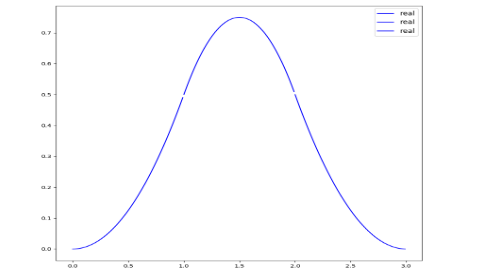
\includegraphics{119.png}

\section*{VI}
Prove :

consider $[t_{i-1}, t_{i}, t_{i+1}, t_{i+2}] = \frac{[t_{i-1}, t_{i}, t_{i+1}] - [t_{i}, t_{i+1}, t_{i+2}]}{t_{i-1} - t_{i+2}}$

Right side :
\begin{align}
    & ([t_{i-1}, t_{i}, t_{i+1}] - [t_{i}, t_{i+1}, t_{i+2}])(t-x)_{+}^{2} \\
    = & \left( \frac{[t_{i+2}, t_{i+1}] - [t_{i+1}, t_{i}]}{t_{i+2} - t_{i}} \right) 
    - \frac{[t_{i+1}, t_{i}] - [t_{i}, t_{i-1}]}{t_{i+1} - t_{i-1}}(t-x)_{+}^{2} \\
    = & \frac{1}{t_{i+2}-t_{i}} \left( \frac{(t_{i+2}-x)_{+}^{2} - (t_{i+1}-x)_{+}^{2}}{t_{i+2} - t_{i+1}} 
    - \frac{(t_{i+1}-x)_{+}^{2} - (t_{i}-x)_{+}^{2}}{t_{i+1} - t_{i}} \right) \\
    & - \frac{1}{t_{i+1}-t_{i-1}} \left( \frac{(t_{i+1}-x)_{+}^{2} - (t_{i}-x)_{+}^{2}}{t_{i+1}-t_{i}} 
    - \frac{(t_{i}-x)_{+}^{2} - (t_{i-1}-x)_{+}^{2}}{t_{i}-t_{i-1}} \right) \\
    = & B_{i}^{2}(x) =
    \left\{
    \begin{array}{rl}
        & \frac{(x-t_{i-1}^{2})}{(t_{i+1}-t_{i-1})(t_{i}-t_{i-1})} , \hspace{3cm} x \in (t_{i-1}, t_{i}] \\
        & \frac{(x - t_{i-1})(t_{i+1} - x)}{(t_{i+1}-t_{i-1})(t_{i+1}-t_{i})} 
        + \frac{(x - t_{i})(t_{i+2} - x)}{(t_{i+2}-t_{i})(t_{i+1}-t_{i})} , \hspace{0.5cm} x \in (t_{i}, t_{i+1}] \\
        & \frac{(t_{i+2} - x)^{2}}{(t_{i+2}-t_{i})(t_{i+2}-t_{i+1})} , \hspace{3cm} x \in (t_{i+1}, t_{i+2}] \\
    \end{array}
    \right.  % 添加对应的右侧分隔符
\end{align}



\section*{VII}
Prove :

According to the theroem3.34, $\frac{d}{dx}B_{i}^{n}(x) = \frac{nB_{i}^{n-1}}{t_{i+n-1} - t_{i-1}} - \frac{nB_{i+1}^{n-1}(x)}{t_{i+n}-t_{i}}$
we integrate the both side of equal ,we have 
$\int_{t_{i-1}}^{i+n} \frac{d}{dx}B_{i}^{n}(x) \,dx = \int_{t_{i-1}}^{t_{i+n}} \frac{nB_{i}^{n-1}}{t_{i+n-1} - t_{i-1}} - \frac{nB_{i+1}^{n-1}(x)}{t_{i+n}-t_{i}} \,dx $

Left side $= B_{i}^{n}(t_{i+n}) - B_{i}^{n}(t_{i-1}) = 0 - 0 = 0$
Right side :for any $x \in [t_{i+n-1}, t_{i+n}]$, we have $B_{i}^{n-1}(x) = 0$, and also $B_{i}^{n-1}(t_{i-1}) = 0$,
$\int_{t_{i-1}}^{t_{i+n}} \frac{nB_{i}^{n-1}}{t_{i+n-1} - t_{i-1}} \,dx 
= \int_{t_{i-1}}^{t_{i+n-1}} \frac{nB_{i}^{n-1}(x)}{t_{i+n-1} - t_{i-1}} \,dx $.

similarly, 
$\int_{t_{i-1}}^{t_{i+n}} \frac{nB_{i+1}^{n-1}(x)}{t_{i+n}-t_{i}} \,dx 
= \int_{t_{i}}^{t_{i+n}} \frac{nB_{i+1}^{n-1}(x)}{t_{i+n} - t_{i}} \,dx $

So, $\int_{t_{i-1}}^{t_{i+n-1}} \frac{nB_{i}^{n-1}(x)}{t_{i+n-1} - t_{i-1}} \,dx 
= \int_{t_{i}}^{t_{i+n}} \frac{nB_{i+1}^{n-1}(x)}{t_{i+n} - t_{i}} \,dx $

\section*{VIII}

\subsection*{VIII-a}
Prove :

m = 4, n = 2.We need to verify that $\tau_{2}(x_{i}, x_{i+1}, x_{i+2}) = [x_{i}, x_{i+1}, x_{i+2}]x^{4}$
Left : $\tau_{2}(x_{i}, x_{i+1}, x_{i+2}) = x_{i}^{2} + x_{i+1}^{2} + x_{i+2}^{2} + x_{i}x_{i+1} + x_{i+1}x_{i+2} + x_{i+2}x_{i}$

Right : \begin{align}
    [x_{i}, x_{i+1}, x_{i+2}]x^{4} &= \frac{(x_{i} + x_{i+1})(x_{i}^{2} + x_{i+1}^{2})
        - (x_{i+1} + x_{i+2})(x_{i+1}^{2} + x_{i+2}^{2})}{x_{i} - x_{i+2}} \\
    &= \frac{(x_{i-2} - x_{i})(x_{i+2}^{2} + x_{i}x_{i+2} + x_{i}^{2}) + x_{i+1}^{2}(x_{i+2} - x_{i})
        + x_{i+1}(x_{i+2} - x_{i})(x_{i+2}^{2} + x_{i})}{x_{i+2} - x_{i}} \\
    &= \tau_{2}(x_{i}, x_{i+1}, x_{i+2})\\
    \end{align}


\subsection*{VIII-b}
Prove is similarly to the Theorem 3.46 :

By Lemma 3.45, we have,
\begin{align}
    (x_{n+1} - x_{1})\tau_{k}(x_{1},\cdots,x_{n+1}) 
    &= \tau_{k+1}(x_{1},\cdots,x_{n+1}) - \tau_{k}(x_{1},\cdots,x_{n}) - x_{1}\tau_{k}(x_{1},\cdots,x_{n+1})\\
    &= \tau_{k+1}(x_{1},\cdots,x_{n+1}) + x_{1}\tau_{k}(x_{1},\cdots,x_{n+1}) \\
    &- \tau_{k+1}(x_{1},\cdots,x_{n}) - x_{1}\tau_{k}(x_{1},\cdots,x_{n+1}) \\
    &= \tau_{k+1}(x_{2},\cdots,x_{n+1}) + \tau_{k+1}(x_{1},\cdots,x_{n}) \\
\end{align}

the rest of prove is an induction on n.
For n = 0, it is obvious that $\tau_{m}(x_{i}) = [x_{i}]x^{m}$ 
Now suppose above holds of nonnegative integer n < m.Then the induction hypothesis yields,
\begin{align}
    &\tau_{m-n-1}(x_{i},\cdots,x_{i+n+1})\\
    =&\frac{\tau_{m-n}(x_{i+1},\cdots,x_{i+n+1}) - \tau_{m-n}(x_{i},\cdots,x_{i+n})}{x_{i+n+1} - x_{i}}\\
    =&\frac{[x_{i+1},\cdots,x_{i+n+1}]x^{m}-[x_{i},\cdots,x_{i+n}]x^{m}}{x_{i+n+1} - x_{i}}\\
    =&[x_{i},\cdots,x_{i+n+1}]x^{m}
\end{align}

\begin{flushright} 
    $\square$ 
\end{flushright} 

% ===============================================
\section*{ \center{\normalsize {Acknowledgement}} }
Give your acknowledgements here(if any).

\end{document}